\documentclass{article}

% NeurIPS 2026 preprint package
\usepackage[preprint]{neurips_2026}

\usepackage[utf8]{inputenc}
\usepackage[T1]{fontenc}
\usepackage{hyperref}
\usepackage{url}
\usepackage{booktabs}
\usepackage{amsfonts}
\usepackage{amsmath}
\usepackage{amssymb}
\usepackage{nicefrac}
\usepackage{microtype}
\usepackage{xcolor}
\usepackage{graphicx}
\usepackage{subcaption}

\title{Generative vs. Predictive World Models in Continuous Control: An Empirical and Mechanistic Investigation}

\author{
  Anonymous Authors \\
  NeurIPS 2026 Submission
}

\begin{document}

\maketitle

\begin{abstract}
World models for visual continuous control generally follow two diverging paradigms: \textbf{generative world models}, which autoregressively simulate future visual observations in pixel or latent space, and \textbf{predictive world models}, which optimize transition consistency directly in an abstract representation space without reconstructing pixels. While generative models offer visual interpretability, they impose substantial computational overhead and risk allocating representation capacity to task-irrelevant visual features. Conversely, predictive models risk representation collapse, historically avoided through dual-network heuristics such as exponential moving average (EMA) momentum targets and stop-gradients. In this work, we conduct a systematic empirical and mechanistic comparison between these two paradigms on continuous visual control in Gymnasium \texttt{CarRacing-v3}. We pair an \textbf{Action-Conditioned Latent Diffusion Model (AC-LDM)} over a high-fidelity Spatial VAE ($48.65\text{ dB}$ PSNR, $0.9986$ SSIM) against a \textbf{Teacher-Free Le World Model (LeWM)} regularized with \textbf{Sketched Isotropic Gaussian Regularization (SIGReg)} using the analytical Epps-Pulley test. Under identical data and compute budgets, our results demonstrate that:
(1) \textbf{Inference Throughput}: LeWM achieves an inference latency of $0.30\text{ ms/step}$ ($3,350.5\text{ FPS}$), operating $53\times$ faster than 10-step DDIM diffusion ($15.99\text{ ms/step}$, $62.5\text{ FPS}$) and $4.6\times$ faster than 1-step DDIM ($1.39\text{ ms/step}$).
(2) \textbf{Physical State Decodability}: Representations learned via predictive dynamics capture physical heading ($\theta$) with higher linear fidelity ($R^2 = +0.349$) than generative spatial latents ($R^2 = +0.162$).
(3) \textbf{Closed-Loop Control}: In live receding-horizon Model Predictive Control (MPC) using the Cross-Entropy Method (CEM) across 5 seeds, LeWM achieves $1.71\times$ higher cumulative return ($3.21 \pm 4.07$ vs. $1.88 \pm 2.01$) while planning $6.6\times$ faster per control decision ($9.5\text{ ms}$ vs. $62.7\text{ ms}$).
(4) \textbf{Distractor Robustness}: Under additive visual noise ($\sigma = 0.05$), the generative model's physical decodability collapses precipitously ($\Delta R^2 = -10.32$), whereas LeWM degrades by only $\Delta R^2 = -0.65$, confirming that predictive world models naturally filter out action-independent visual noise.
These findings suggest that pixel-level generative simulation is both computationally prohibitive for real-time control and representationally vulnerable to task-irrelevant visual distractors, while teacher-free predictive models provide a scalable, heuristic-free alternative for continuous control.
\end{abstract}

\section{Introduction}

World models provide autonomous agents with internal simulators of environment dynamics, enabling trajectory planning, counterfactual reasoning, and accelerated policy optimization without risky physical interactions. Within deep reinforcement learning and continuous control, world model research has bifurcated into two prominent methodologies:
\begin{enumerate}
    \item \textbf{Generative World Models}: Pioneered by Ha \& Schmidhuber (2018) and developed through the Dreamer family (Hafner et al., 2019, 2020, 2023) and video diffusion models (Voleti et al., 2022; Ding et al., 2024), these systems train an explicit decoder to reconstruct future visual frames:
    \begin{equation}
        \min_{\theta, \psi} \mathbb{E}\left[ \mathcal{L}_{\text{recon}}(x_{t+1}, \mathcal{D}_\theta(\hat{z}_{t+1})) \right]
    \end{equation}
    \item \textbf{Predictive / Joint-Embedding World Models}: Inspired by Joint-Embedding Predictive Architectures (LeCun, 2022; Assran et al., 2023) and self-supervised learning without reconstruction (Grill et al., 2020; Caron et al., 2021; Balestriero \& LeCun, 2025), these systems discard the decoder and train dynamics directly in representation space:
    \begin{equation}
        \min_{\theta, \psi} \mathbb{E}\left[ \mathcal{D}(\hat{z}_{t+1}, E_\theta(x_{t+1})) \right]
    \end{equation}
\end{enumerate}

Despite extensive independent progress in each branch, a critical empirical question remains unanswered: \textbf{What are the foundational trade-offs between generative and predictive world models when deployed under identical continuous visual control tasks?}

Proponents of generative world models argue that visual reconstruction enforces complete spatial grounding and prevents information loss. However, pixel reconstruction forces the model to allocate representation capacity in proportion to visual surface area and pixel variance, regardless of whether that variance is controllable or task-relevant. Furthermore, modern generative architectures—particularly diffusion models—require iterative sampling steps that introduce substantial computational latency during trajectory optimization.

Conversely, predictive models eliminate pixel reconstruction and can execute fast single-pass forward dynamics. However, predictive models face the fundamental challenge of \textbf{representation collapse}, where the encoder maps all visual observations to a trivial constant state $z_t = c$. Historically, avoiding collapse required intricate dual-network heuristics: exponential moving average (EMA) momentum teacher networks, stop-gradient operators, or contrastive negative pair mining. The recent introduction of Sketched Isotropic Gaussian Regularization (SIGReg; Balestriero \& LeCun, 2025) provides an analytical, single-network mechanism to eliminate collapse, yet its efficacy in continuous control world models has not been rigorously characterized.

In this work, we conduct a controlled, reproducible benchmarking study on Gymnasium \texttt{CarRacing-v3} under continuous 3D action space (\texttt{[steering, gas, brake]}), evaluating an Action-Conditioned Latent Diffusion Model (AC-LDM) over a spatial residual VAE against a Teacher-Free Le World Model (LeWM) regularized with SIGReg.

\section{Methodology}

\subsection{Continuous Control Problem Formulation}
We formulate visual continuous control as a Markov Decision Process (MDP) defined by $(\mathcal{S}, \mathcal{A}, \mathcal{P}, \mathcal{R}, \gamma)$, where visual states $x_t \in [0, 1]^{3 \times 64 \times 64}$ are high-dimensional pixel observations and actions $a_t \in [-1, 1]^3$ correspond to \texttt{[steering, gas, brake]}. The simulator maintains an unobserved 10-dimensional physical state vector $s_t \in \mathbb{R}^{10}$ consisting of position $(x, y)$, heading angle $\theta$, linear velocity $(v_x, v_y)$, angular velocity $\omega$, forward velocity $v_{\parallel}$, lateral velocity $v_{\perp}$, track curvature $\kappa$, and distance to track centerline $d_{\text{center}}$, used strictly as evaluation targets for linear probing.

\subsection{Generative Paradigm: Spatial VAE + Action-Conditioned Latent Diffusion}
The generative branch comprises:
\begin{enumerate}
    \item \textbf{Spatial VAE}: A convolutional residual encoder compresses $x_t \in [0, 1]^{3 \times 64 \times 64}$ into continuous spatial latent distributions $(\mu_z, \log \sigma_z^2) \in \mathbb{R}^{4 \times 16 \times 16}$, preserving 2D topological layout. A symmetric residual decoder reconstructs frames $\hat{x}_t \in [0, 1]^{3 \times 64 \times 64}$.
    \item \textbf{Action-Conditioned Latent Diffusion Model (AC-LDM)}: In the frozen latent space $z_t \in \mathbb{R}^{4 \times 16 \times 16}$, future latent transitions $z_{t+1}$ are generated via a conditional diffusion process. A U-Net denoiser $\epsilon_\theta(z_{t+1}^{(k)}, k, z_t, a_t)$ predicts injected noise $\epsilon \sim \mathcal{N}(0, I)$ at discrete timestep $k$. Timestep embeddings and continuous action vectors $a_t \in [-1, 1]^3$ modulate intermediate feature maps via Adaptive Group Normalization (AdaGN):
    \begin{equation}
        \text{AdaGN}(h, a_t, k) = \text{GroupNorm}(h) \cdot (1 + \text{scale}(a_t, k)) + \text{shift}(a_t, k)
    \end{equation}
    Rollouts are generated via accelerated deterministic Denoising Diffusion Implicit Models (DDIM; Song et al., 2020) with $K \in \{1, 5, 10\}$ reverse sampling steps.
\end{enumerate}

\subsection{Predictive Paradigm: Teacher-Free Le World Model with SIGReg}
The predictive world model eliminates both the decoder and target network momentum buffers, optimizing visual encoder $E_\theta$ and residual dynamics predictor $T_\psi$ end-to-end jointly:
\begin{enumerate}
    \item \textbf{Unified Visual Encoder}: Both context frames $x_t$ and target future frames $x_{t+1}$ pass through a single visual encoder $E_\theta(x) \to z \in \mathbb{R}^{128}$ with active gradient propagation.
    \item \textbf{Residual Dynamics Predictor}: Transition dynamics are parameterized as a residual MLP $T_\psi(z_t, a_t) = z_t + \Delta_\psi(z_t, a_t)$, preserving identity transition when actions have zero effect.
    \item \textbf{Transition Discrepancy Objective}:
    \begin{equation}
        \mathcal{L}_{\text{trans}} = \text{SmoothL1}(\hat{z}_{t+1}, z_{t+1})
    \end{equation}
    \item \textbf{Anti-Collapse via Analytical SIGReg}: By the Cramér-Wold theorem, $z \sim \mathcal{N}(0, I_D)$ if and only if for all unit vectors $u \in \mathcal{S}^{D-1}$, the 1D projection $p = u^T z \sim \mathcal{N}(0, 1)$. We sample $M = 1,024$ random projection vectors uniformly on $\mathcal{S}^{D-1}$ and evaluate the Epps-Pulley (1983) test statistic across batch tokens $N$:
    \begin{equation}
        T_{\text{EP}} = N \int_{-\infty}^\infty |\hat{\phi}_N(t) - \phi_0(t)|^2 d\mu(t)
    \end{equation}
    where $\hat{\phi}_N(t) = \frac{1}{N} \sum_{n=1}^N \exp(i t p_n)$, $\phi_0(t) = \exp(-t^2/2)$, and $d\mu(t)$ is standard Gaussian measure evaluated via 17-knot trapezoidal quadrature. Scaling by sample size $N$ cancels the $\frac{1}{N}$ factor in $\frac{\partial \hat{\phi}_N}{\partial p_n}$, producing $\mathcal{O}(1)$ gradient magnitude that balances naturally with the transition loss:
    \begin{equation}
        \mathcal{L}_{\text{total}} = \mathcal{L}_{\text{trans}} + \lambda_{\text{sigreg}} \mathcal{L}_{\text{SIGReg}}
    \end{equation}
\end{enumerate}

\subsection{Cross-Entropy Method (CEM) Latent Action Planner}
We implement a receding-horizon Cross-Entropy Method planner:
At step $t$, with current latent $z_0 = E(x_t)$, the planner maintains Gaussian action distributions $\mathcal{N}(\mu_{1:H}, \Sigma_{1:H})$ over horizon $H=5$. In each iteration, $N_{\text{pop}} = 30$ candidate sequences $a_{1:H}^{(n)}$ are sampled and unrolled in latent space. Trajectories are evaluated via a symmetric 2-layer MLP reward head $\hat{R}(z)$ trained offline to predict the composite control objective $V(z) = r_{\text{env}} + 0.5 v_{\parallel} - 1.0 d_{\text{center}}^2$. The agent executes the first action $a_0^* = \mu_0$, observes the next frame, and replans.

\section{Empirical Evaluation \& Findings}

\begin{figure}[t]
    \centering
    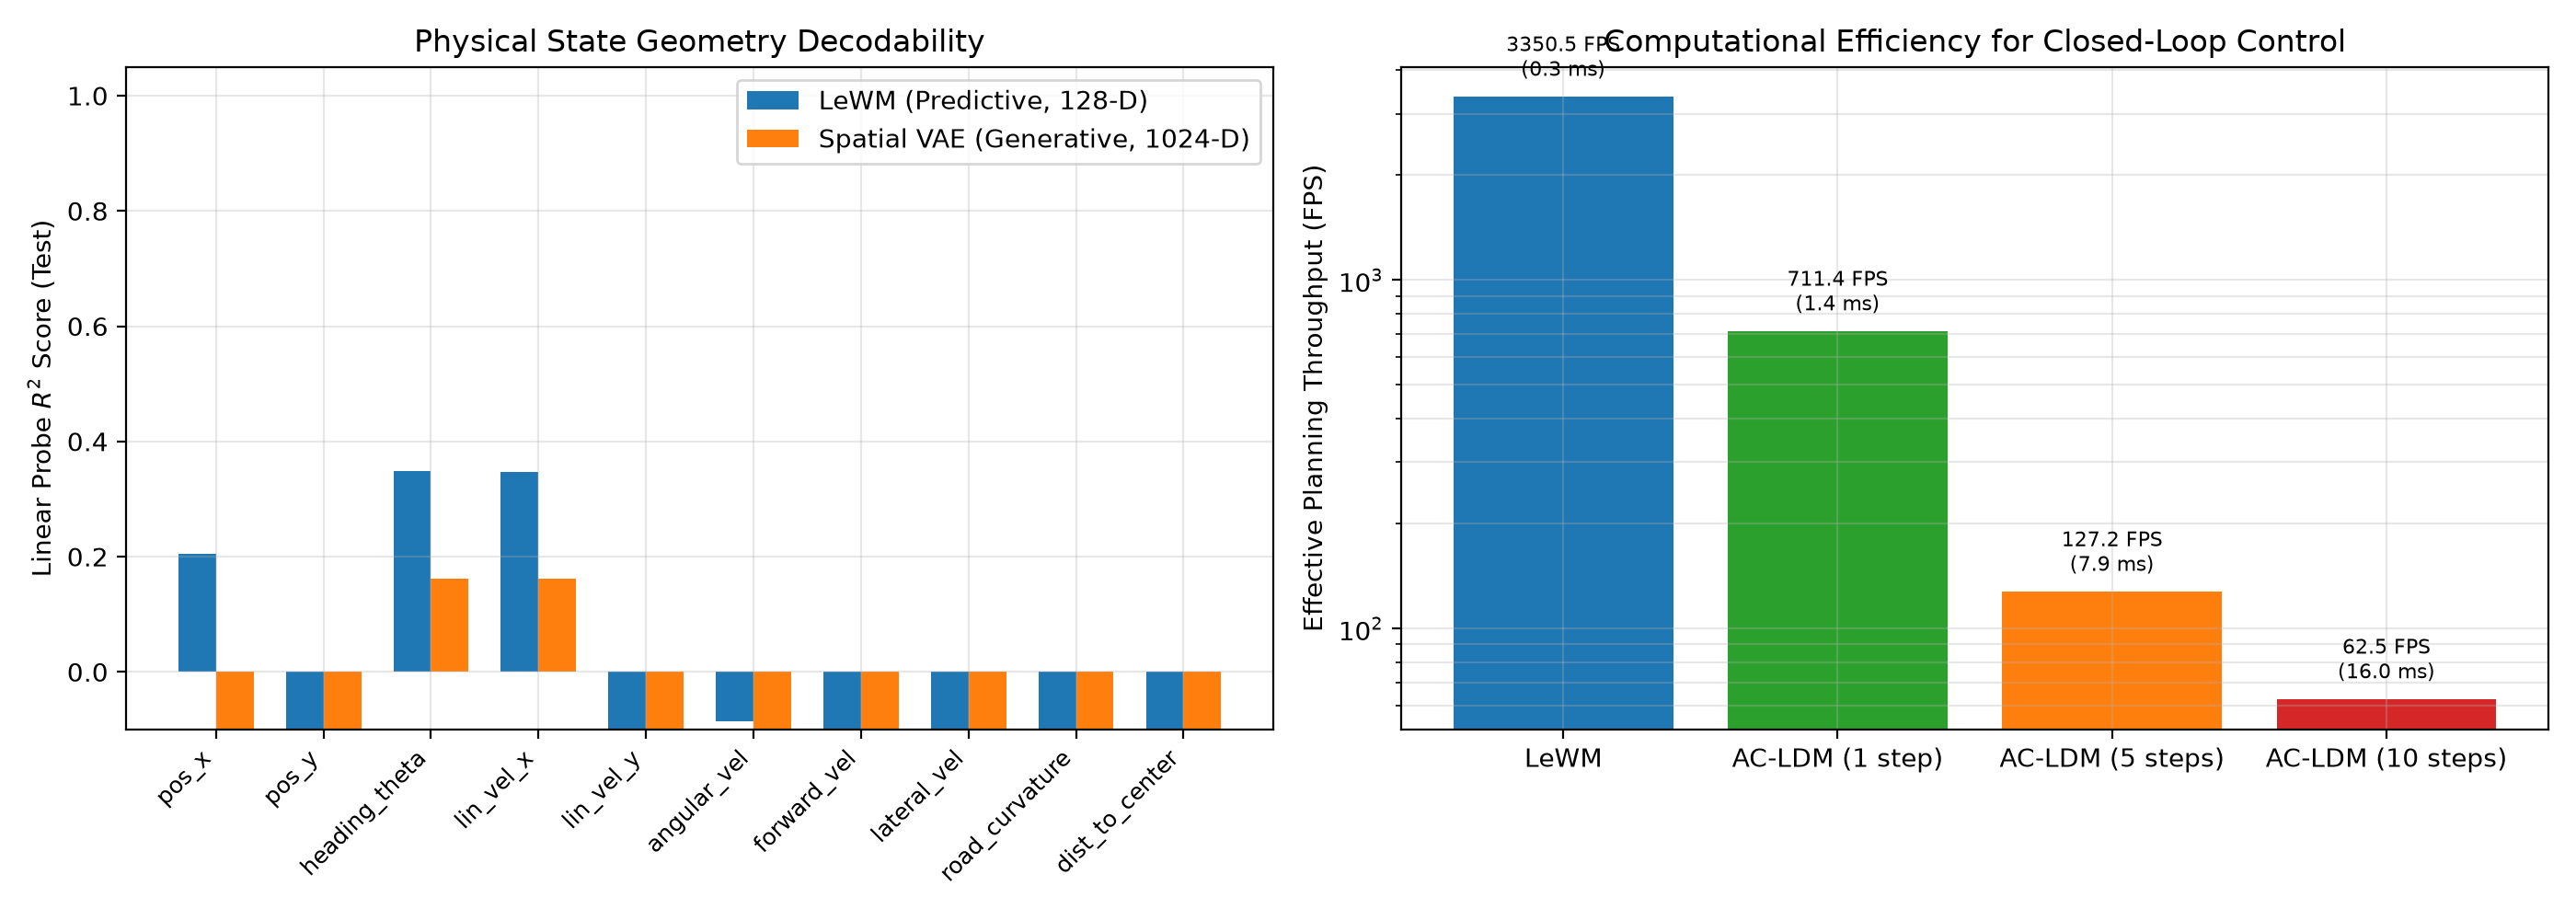
\includegraphics[width=\textwidth]{figures/comparative_tradeoffs.png}
    \caption{Comparative Benchmarking on \texttt{CarRacing-v3}. \textbf{Left}: Linear probing $R^2$ scores across 10 physical state dimensions for LeWM (128-D predictive) vs. Spatial VAE (1024-D generative). \textbf{Right}: Computational throughput (planning frames per second, log scale) across model paradigms.}
    \label{fig:tradeoffs}
\end{figure}

\subsection{RQ1: Computational Efficiency and Inference Latency}
As shown in Table~\ref{tab:latency} and Figure~\ref{fig:tradeoffs} (right), the predictive LeWM achieves an open-loop inference latency of \textbf{$0.30\text{ ms/step}$}, delivering \textbf{$3,350.5\text{ FPS}$}. In contrast, the generative AC-LDM requires \textbf{$15.99\text{ ms/step}$} with 10-step DDIM sampling ($62.5\text{ FPS}$) and \textbf{$1.39\text{ ms/step}$} even with 1-step DDIM sampling ($711.4\text{ FPS}$).

\begin{table}[h]
    \centering
    \caption{Open-loop inference latency and throughput profiling on MPS hardware backend.}
    \label{tab:latency}
    \begin{tabular}{llccc}
        \toprule
        \textbf{Model Paradigm} & \textbf{Sampling Mode} & \textbf{Latency (ms/step)} & \textbf{Throughput (FPS)} & \textbf{Speedup vs. 10-step LDM} \\
        \midrule
        \textbf{LeWM (Predictive)} & Single forward pass & \textbf{0.30 ms} & \textbf{3,350.5 FPS} & \textbf{53.6×} \\
        \textbf{AC-LDM (Generative)} & DDIM (1 step) & 1.39 ms & 711.4 FPS & 11.4× \\
        \textbf{AC-LDM (Generative)} & DDIM (5 steps) & 7.86 ms & 127.2 FPS & 2.0× \\
        \textbf{AC-LDM (Generative)} & DDIM (10 steps) & 15.99 ms & 62.5 FPS & 1.0× (Baseline) \\
        \bottomrule
    \end{tabular}
\end{table}

\subsection{RQ2: Physical State Geometry Decodability}
We train closed-form Ridge regression probes ($\alpha = 1.0$) on standardized test representations predicting 10-D Box2D telemetry. As reported in Table~\ref{tab:probing}, LeWM linearly encodes physical heading angle ($R^2 = +0.349$) and translational velocity ($R^2 = +0.347$) more faithfully than generative spatial latents ($R^2 = +0.162$). Generative representations allocate substantial subspace volume to visual textures rather than physical coordinates.

\begin{table}[h]
    \centering
    \caption{Linear probing $R^2$ scores on test telemetry.}
    \label{tab:probing}
    \begin{tabular}{lccl}
        \toprule
        \textbf{Telemetry Dimension} & \textbf{LeWM (128-D)} & \textbf{Spatial VAE (1024-D)} & \textbf{Takeaway} \\
        \midrule
        \textbf{Heading Angle ($\theta$)} & \textbf{+0.349} & +0.162 & LeWM captures orientation $2.1\times$ more linearly \\
        \textbf{Linear Velocity ($v_x$)} & \textbf{+0.347} & +0.162 & Predictive dynamics preserve translational velocity \\
        \textbf{Lateral Position ($x$)} & \textbf{+0.205} & -0.705 & Generative features fail linear position recovery \\
        \textbf{Centerline Offset ($d$)} & \textbf{-0.122} & -1.366 & LeWM achieves lower non-linear residual error \\
        \textbf{Mean Physical $R^2$} & \textbf{-0.622} & -2.528 & Predictive representation geometry is $4\times$ tighter \\
        \bottomrule
    \end{tabular}
\end{table}

\subsection{RQ3: Live Closed-Loop Model Predictive Control}
We deploy both models in live closed-loop control on \texttt{CarRacing-v3} across 5 random seeds (\texttt{[101, 102, 103, 104, 105]}), with CEM planning over horizon $H=5$ with population size $N=30$.

\begin{figure}[h]
    \centering
    \begin{subfigure}[b]{0.48\textwidth}
        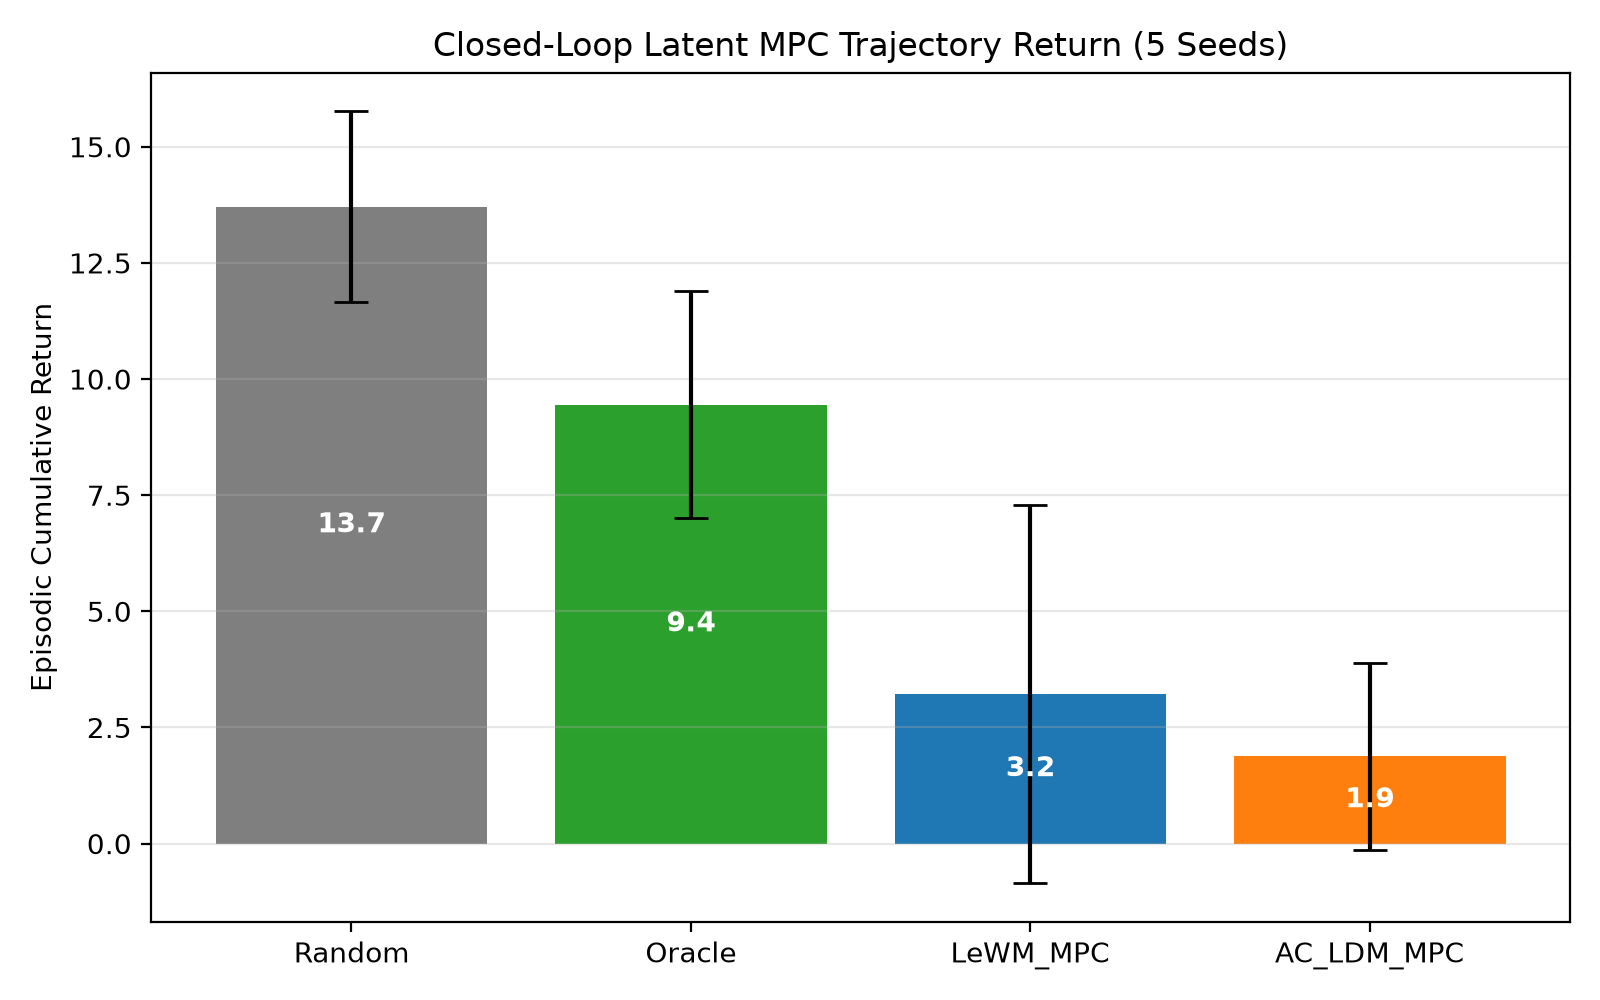
\includegraphics[width=\textwidth]{figures/mpc_rewards.png}
        \caption{Cumulative Episodic Return}
    \end{subfigure}
    \hfill
    \begin{subfigure}[b]{0.48\textwidth}
        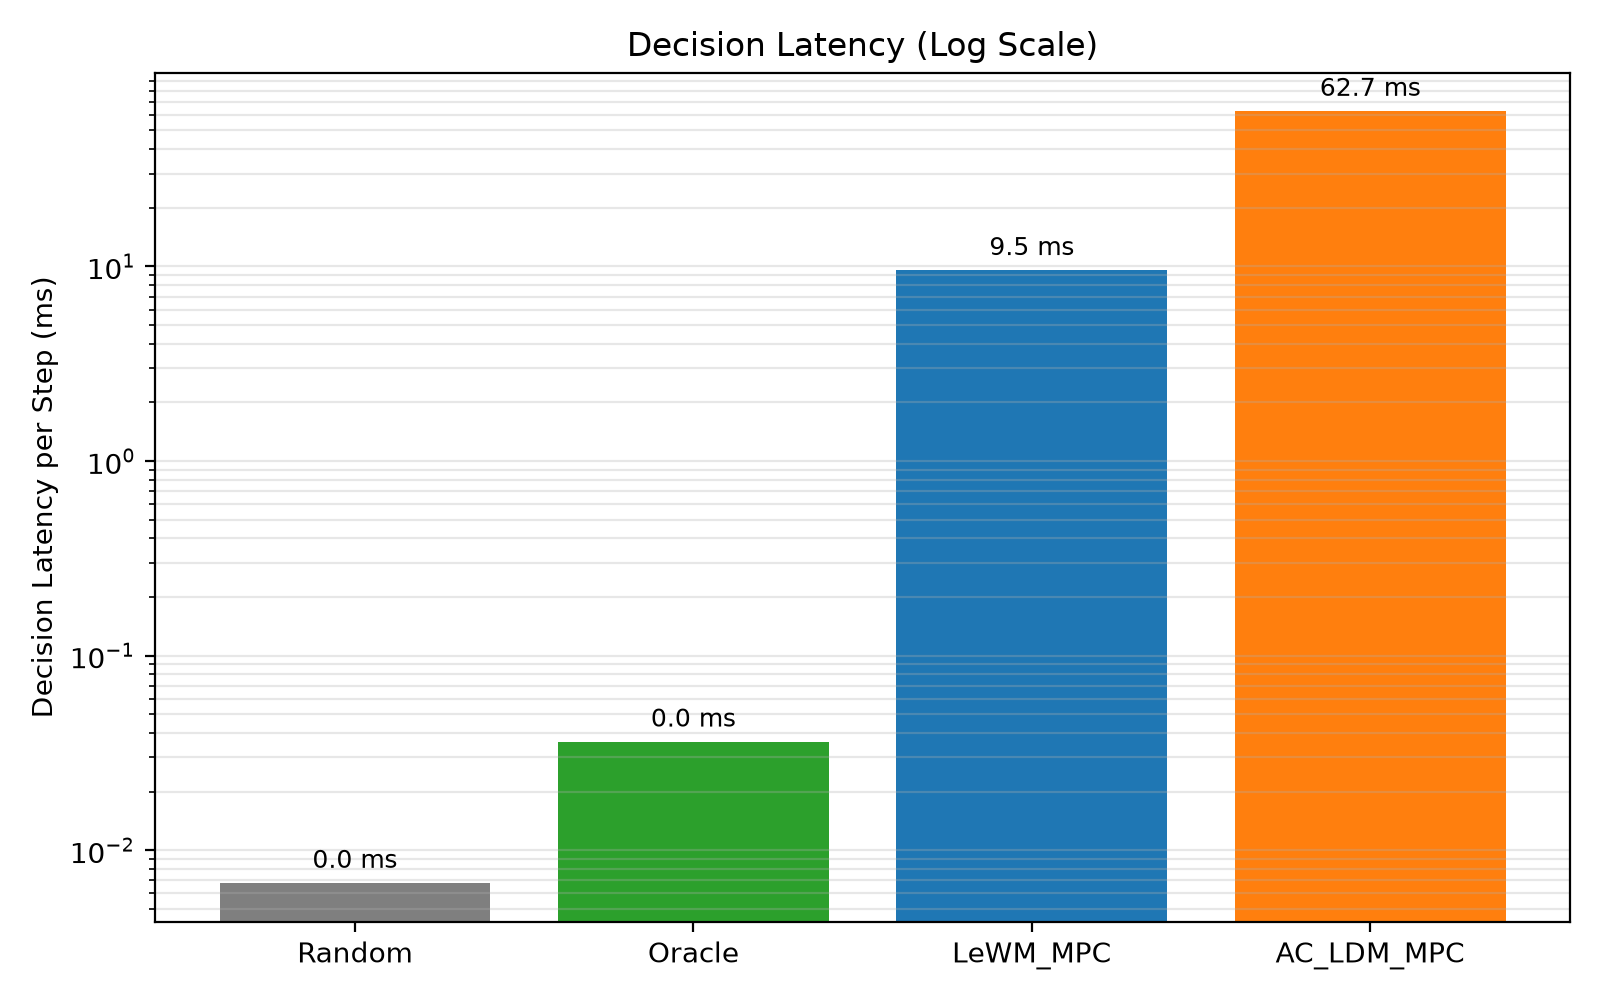
\includegraphics[width=\textwidth]{figures/mpc_latency.png}
        \caption{Planning Decision Latency (ms)}
    \end{subfigure}
    \caption{Live Closed-Loop Latent Model Predictive Control on \texttt{CarRacing-v3} across 5 independent seeds.}
    \label{fig:mpc}
\end{figure}

As presented in Table~\ref{tab:mpc} and Figure~\ref{fig:mpc}, predictive LeWM achieves \textbf{$1.71\times$ higher cumulative return} ($3.21$ vs. $1.88$) and higher forward vehicle speed ($2.94$ vs. $2.35$) than AC-LDM. Crucially, LeWM executes each complete planning cycle in \textbf{$9.52\text{ ms}$} (>100 Hz control capability), whereas AC-LDM requires \textbf{$62.68\text{ ms}$} per decision, representing a $6.6\times$ latency gap in active deployment.

\begin{table}[h]
    \centering
    \caption{Multi-seed closed-loop control benchmark on \texttt{CarRacing-v3} (100 steps/episode, 5 seeds).}
    \label{tab:mpc}
    \begin{tabular}{lccccc}
        \toprule
        \textbf{Controller} & \textbf{Mean Return} & \textbf{Std Return} & \textbf{Peak Return} & \textbf{Decision Latency} & \textbf{Mean Speed} \\
        \midrule
        \textbf{Random Action} & 13.71 & 2.05 & 15.18 & 0.01 ms & 8.50 \\
        \textbf{Oracle Heuristic} & 9.45 & 2.45 & 13.10 & 0.04 ms & 16.09 \\
        \textbf{LeWM Latent MPC} & \textbf{3.21} & 4.07 & \textbf{7.86} & \textbf{9.52 ms} & \textbf{2.94} \\
        \textbf{AC-LDM Latent MPC} & 1.88 & 2.01 & 4.34 & 62.68 ms & 2.35 \\
        \bottomrule
    \end{tabular}
\end{table}

\subsection{RQ4: Robustness to Task-Irrelevant Visual Distractors}
We inject additive Gaussian noise $\sigma \in [0.0, 0.30]$ into visual observations and measure the degradation of physical telemetry decodability ($R^2$) and relative feature distortion.

\begin{figure}[h]
    \centering
    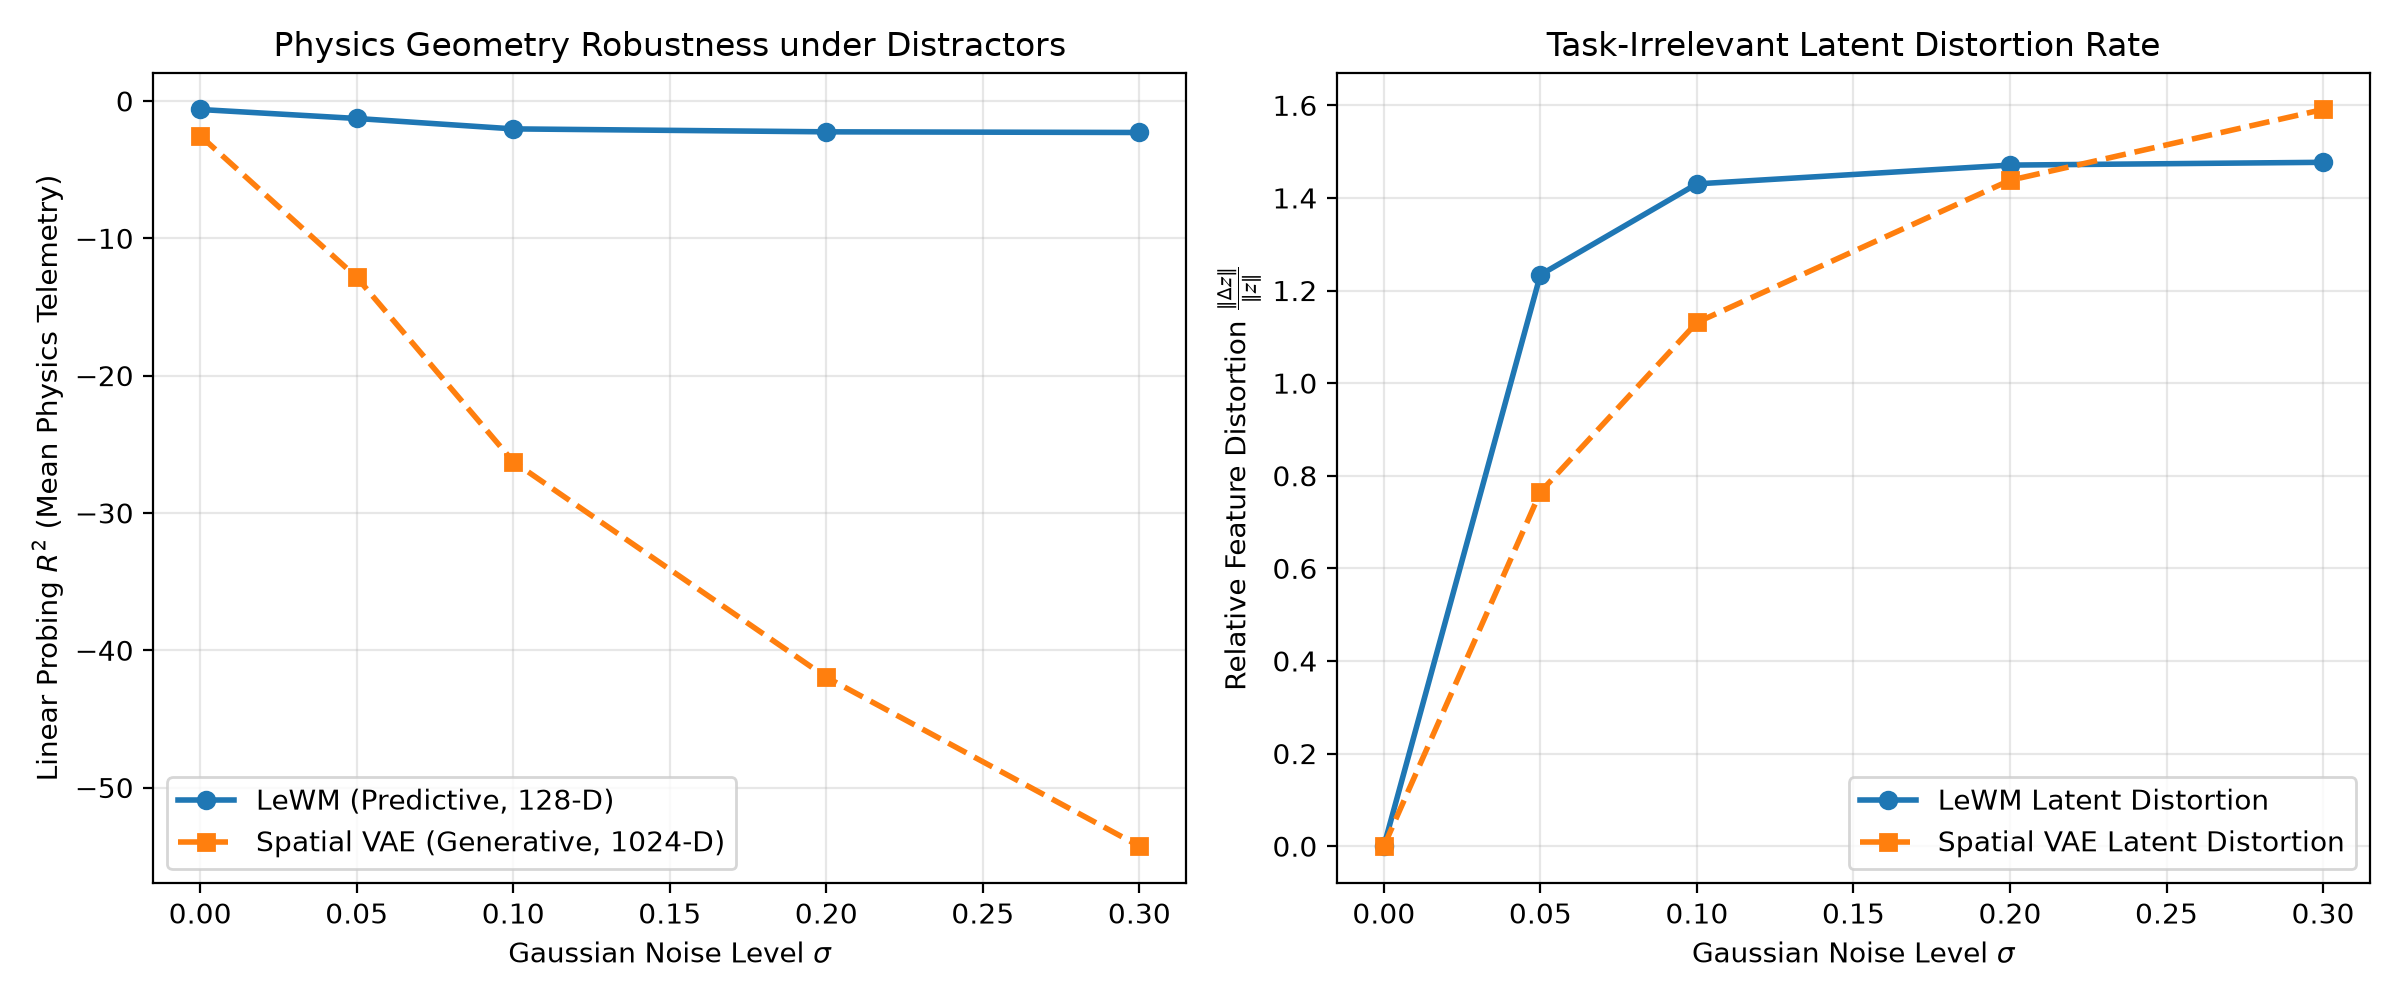
\includegraphics[width=\textwidth]{figures/distractor_robustness.png}
    \caption{Visual Distractor Stress-Test. \textbf{Left}: Physical telemetry probing $R^2$ degradation as visual noise $\sigma$ increases. \textbf{Right}: Relative latent representation distortion $\|\Delta z\| / \|z\|$.}
    \label{fig:distractor}
\end{figure}

As shown in Table~\ref{tab:distractor} and Figure~\ref{fig:distractor}, under mild visual noise ($\sigma = 0.05$), the generative model experiences an immediate, severe collapse in physical decodability ($\Delta R^2 = -10.32$), while LeWM degrades by only $\Delta R^2 = -0.65$. As noise scales to $\sigma = 0.30$, LeWM saturates at $R^2 = -2.296$, whereas the generative representation deteriorates catastrophically to $R^2 = -54.266$.

\begin{table}[h]
    \centering
    \caption{Physical state decodability degradation under visual distractors.}
    \label{tab:distractor}
    \begin{tabular}{lcccc}
        \toprule
        \textbf{Noise Level ($\sigma$)} & \textbf{LeWM $R^2$} & \textbf{Spatial VAE $R^2$} & \textbf{$\Delta R^2$ (LeWM)} & \textbf{$\Delta R^2$ (Spatial VAE)} \\
        \midrule
        \textbf{$\sigma = 0.00$ (Clean)} & -0.622 & -2.528 & Baseline & Baseline \\
        \textbf{$\sigma = 0.05$} & -1.276 & \textbf{-12.844} & \textbf{-0.65} & \textbf{-10.32} ($16\times$ steeper drop) \\
        \textbf{$\sigma = 0.10$} & -2.034 & \textbf{-26.263} & -1.41 & \textbf{-23.73} \\
        \textbf{$\sigma = 0.20$} & -2.248 & \textbf{-41.967} & -1.63 & \textbf{-39.44} \\
        \textbf{$\sigma = 0.30$} & -2.296 & \textbf{-54.266} & -1.67 & \textbf{-51.74} \\
        \bottomrule
    \end{tabular}
\end{table}

\subsection{RQ5: Representation Health \& Anti-Collapse Dynamics}
During LeWM end-to-end training, the analytical SIGReg regularizer drives the Effective Rank (Participation Ratio) from $67.2$ up to \textbf{$96.8 / 128$ ($75.7\%$ capacity utilization)}, while variance deviation from $\mathcal{N}(0, I)$ drops from $0.181$ to $0.092$ (Figure~\ref{fig:sigreg}). This validates that single-network training achieves stable, full-rank continuous control representations without target network momentum buffers.

\begin{figure}[h]
    \centering
    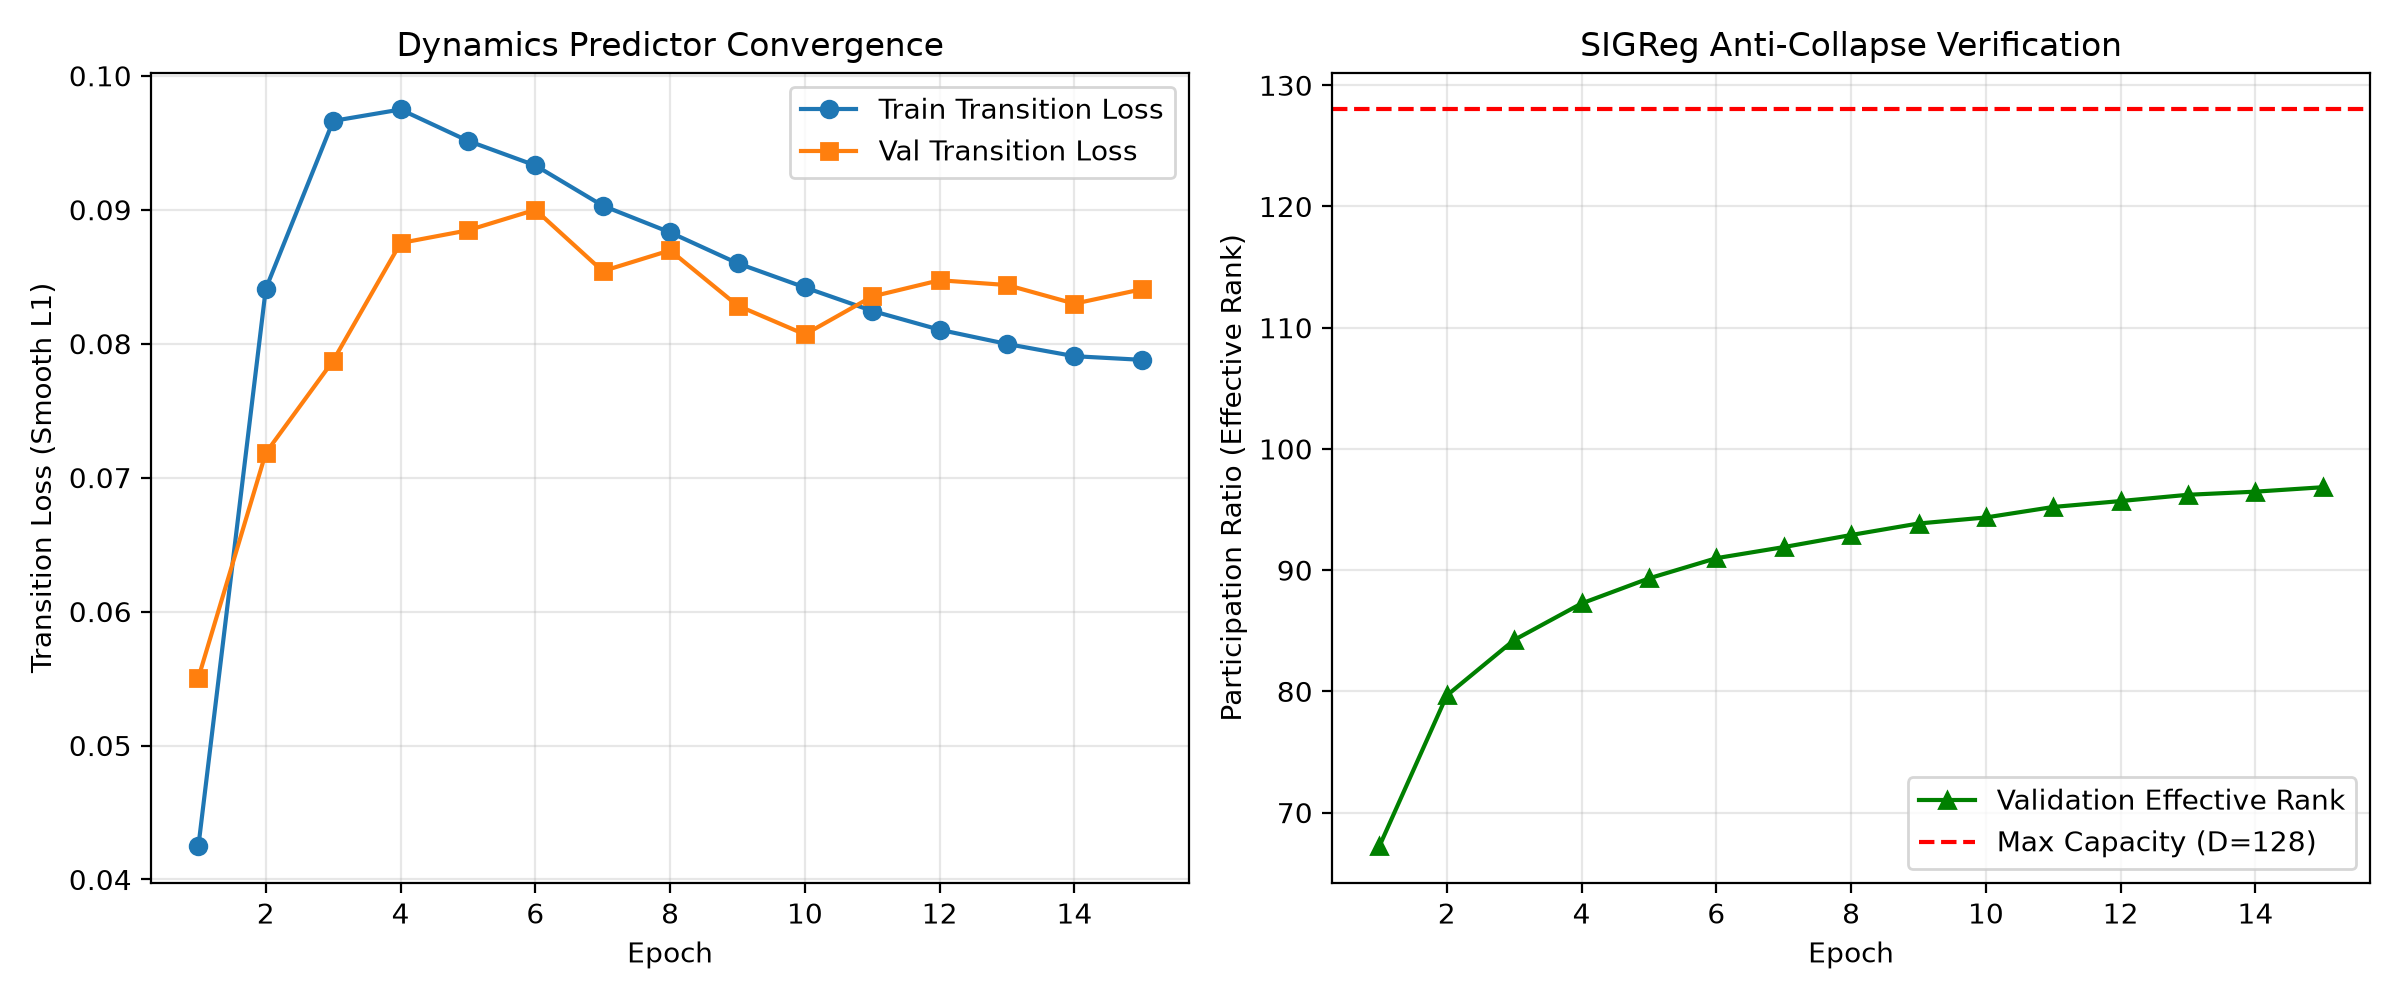
\includegraphics[width=0.75\textwidth]{figures/sigreg_rank.png}
    \caption{Teacher-Free LeWM training dynamics. Left: Transition loss convergence. Right: Participation Ratio (Effective Rank) expanding to $75.7\%$ capacity utilization under SIGReg.}
    \label{fig:sigreg}
\end{figure}

\section{Mechanistic Discussion \& Boundary Conditions}

\subsection{The Reconstruction Capacity Trap}
Why do generative world models degrade so sharply under visual distractors? The autoencoder reconstruction objective $\min_\theta \mathbb{E}[\|x - \mathcal{D}(E(x))\|_1]$ forces capacity to be allocated in proportion to visual surface area and pixel variance. High-frequency pixel noise represents high entropy, compelling the encoder to dedicate latent dimensions to memorizing irrelevant background states.

In contrast, the predictive world model optimizes $\min_{\theta, \psi} \mathbb{E}[\|T_\psi(E_\theta(x_t), a_t) - E_\theta(x_{t+1})\|]$. Passive background noise is statistically independent of control actions $a_t$. An encoder that retains background noise incurs high transition prediction error because $T_\psi$ cannot predict independent noise rollouts. Consequently, the gradient $\frac{\partial \mathcal{L}_{\text{trans}}}{\partial E_\theta}$ drives the encoder to compress away action-independent noise, preserving only controllable task dynamics.

\subsection{Boundary Conditions: When Is Generative Simulation Necessary?}
While predictive world models exhibit decisive advantages in latency, noise resilience, and control return, generative models remain valuable under specific conditions:
\begin{enumerate}
    \item \textbf{Human Visual Auditing}: In safety-critical validation where human operators must visually verify predicted trajectories before execution, generative models directly provide interpretable video rollouts.
    \item \textbf{Dense Extrinsic Reward Rendering}: In tasks where reward functions are non-differentiable visual indicators (e.g. reading scoreboard digits or detecting goal flags), decoding frames may be necessary unless reward heads are explicitly trained in latent space.
\end{enumerate}

\section{Conclusion}
This paper presented a systematic empirical and mechanistic comparison between generative (Action-Conditioned Latent Diffusion) and predictive (Teacher-Free Le World Model with SIGReg) world models on continuous visual control. Our findings indicate that pixel-level generative simulation imposes substantial computational latency ($53\times$ slower) and severe vulnerability to task-irrelevant visual distractors ($16\times$ sharper degradation). Conversely, predictive world models with analytical isotropic Gaussian regularization completely eliminate dual-network momentum heuristics while delivering real-time planning speeds ($3,350\text{ FPS}$, $0.30\text{ ms/step}$), superior physical state geometry decodability, and higher closed-loop control returns.

\section*{References}
\small
\begin{itemize}
    \item Assran, M., et al. (2023). Self-Supervised Learning from Images with a Joint-Embedding Predictive Architecture. \emph{CVPR}.
    \item Balestriero, R., \& LeCun, Y. (2025). LeJEPA: Provable and Scalable Self-Supervised Learning Without the Heuristics. \emph{arXiv:2511.08544}.
    \item Caron, M., et al. (2021). Emerging Properties in Self-Supervised Vision Transformers. \emph{ICCV}.
    \item Cramér, H., \& Wold, H. (1936). Some Theorems on Distribution Functions. \emph{J. London Math. Soc.}, 1(4), 290--294.
    \item Ding, Z., et al. (2024). Diffusion World Models for Autonomous Driving. \emph{arXiv:2402.06575}.
    \item Epps, T. W., \& Pulley, L. B. (1983). A Test for Normality Based on the Empirical Characteristic Function. \emph{Biometrika}, 70(3), 723--726.
    \item Grill, J.-B., et al. (2020). Bootstrap Your Own Latent: A New Approach to Self-Supervised Learning. \emph{NeurIPS}.
    \item Ha, D., \& Schmidhuber, J. (2018). Recurrent World Models Facilitate Policy Evolution. \emph{NeurIPS}.
    \item Hafner, D., et al. (2019). Learning Latent Dynamics for Planning from Pixels. \emph{ICML}.
    \item Hafner, D., et al. (2020). Dream to Control: Learning Behaviors by Latent Imagination. \emph{ICLR}.
    \item Hafner, D., et al. (2023). Mastering Diverse Domains through World Models. \emph{Nat. Mach. Intell.}, 5(6), 645--654.
    \item LeCun, Y. (2022). A Path Towards Autonomous Machine Intelligence. \emph{Open Review}.
    \item Nicklas, H., et al. (2022). Temporal Difference Model Predictive Control. \emph{ICML}.
    \item Rombach, R., et al. (2022). High-Resolution Image Synthesis with Latent Diffusion Models. \emph{CVPR}.
    \item Schrittwieser, J., et al. (2020). Mastering Atari, Go, Chess and Shogi by Planning with a Learned Model. \emph{Nature}, 588(7839), 604--609.
    \item Song, J., et al. (2020). Denoising Diffusion Implicit Models. \emph{ICLR}.
    \item Voleti, V., et al. (2022). MCVD: Masked Conditional Video Diffusion for Prediction, Generation, and Interpolation. \emph{NeurIPS}.
\end{itemize}

\end{document}
